\documentclass{article}
\usepackage[utf8]{inputenc}
\usepackage{tabularx} % extra features for tabular environment
\usepackage{amsmath}  % improve math presentation
\usepackage{graphicx} % takes care of graphic including machinery
\usepackage{xspace}
\usepackage{tikz}
\usepackage{enumitem}
\usetikzlibrary{babel}
\usepackage[american]{circuitikz}
\usetikzlibrary{calc}
\usepackage{float}
\usepackage{siunitx}
\usepackage{pgfplots}
\usepackage[skins,theorems]{tcolorbox}
\tcbset{highlight math style={enhanced,
  colframe=red,colback=white,arc=0pt,boxrule=1pt}}
\pgfplotsset{width=10cm,compat=1.9}
\usepackage[margin=1in,letterpaper]{geometry} % decreases margins
\usepackage{cite} % takes care of citations
\usepackage[final]{hyperref} % adds hyper links inside the generated PDF file
\hypersetup{
colorlinks=true,       % false: boxed links; true: colored links
linkcolor=blue,        % color of internal links
citecolor=blue,        % color of links to bibliography
filecolor=magenta,     % color of file links
urlcolor=blue        
}

\begin{document}

\title{{\textbf{MINI PROJECT 1}}}
\author{\textbf{TADIPATRI UDAY KIRAN REDDY}\\\textbf{EE19BTECH11038}}
\maketitle

\section*{\hfil Calculations}
We need a step-down matching network to match 250 $\si{\ohm}$ to 50 $\si{\ohm}$.\\
\begin{gather*}
	Q = \sqrt{\frac{250}{50} - 1} \implies \tcbhighmath[drop fuzzy shadow]{Q = 2}\\
	Q = \frac{\omega L}{50} \implies \tcbhighmath[drop fuzzy shadow]{L = 15.9nH}\\
	Q = \omega C250 \implies \tcbhighmath[drop fuzzy shadow]{C = 1.2pF}
\end{gather*}
\section*{\hfil On chip inductor design}
Inductor design is done on ASITIC CAD tool. Using \textbf{Square Symmetric Spiral} with the below specifications.\\
\begin{figure}[H]
	\centering
	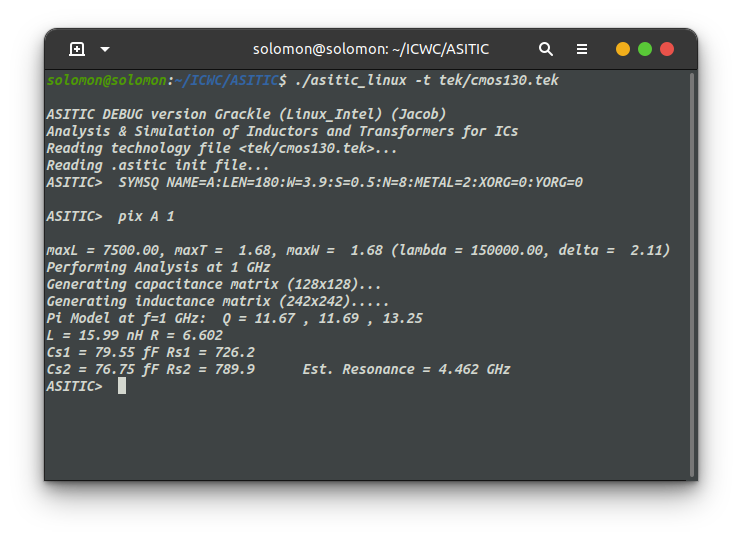
\includegraphics[scale=0.5]{./figs/pix.png}
\end{figure}
The Pi Model parameters are ,\\
$\mathbf{L=15.99nF, R=6.602\si{\ohm}, Cs1=79.55fF, Rs1=726.2\si{\ohm}, Cs2=76.75fF, Rs2=789.9\si{\ohm}}$.
\begin{figure}[H]
	\centering
	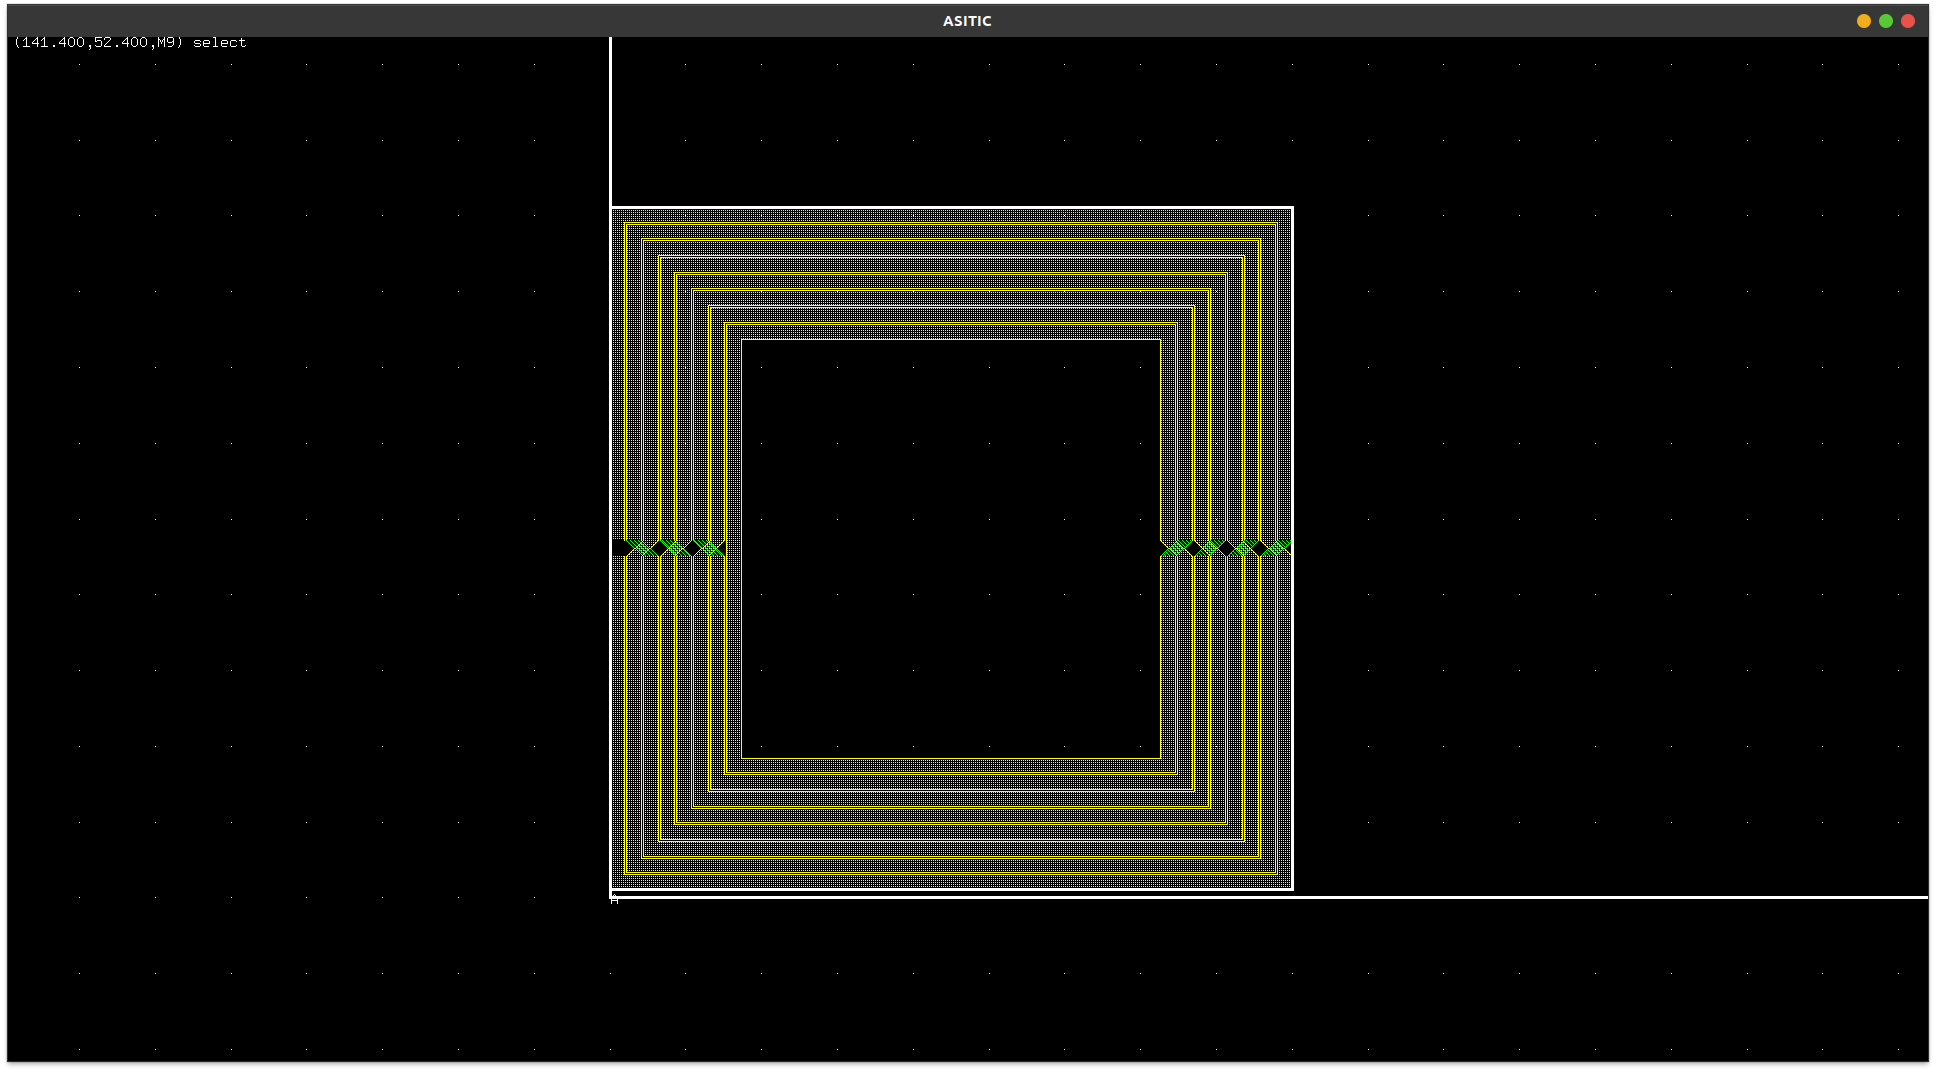
\includegraphics[scale=0.3]{./figs/ind.png}
\end{figure}
\section*{\hfil Schematic}
Both ideal and non-ideal networks are simulated and compared.
\begin{figure}[H]
	\centering
	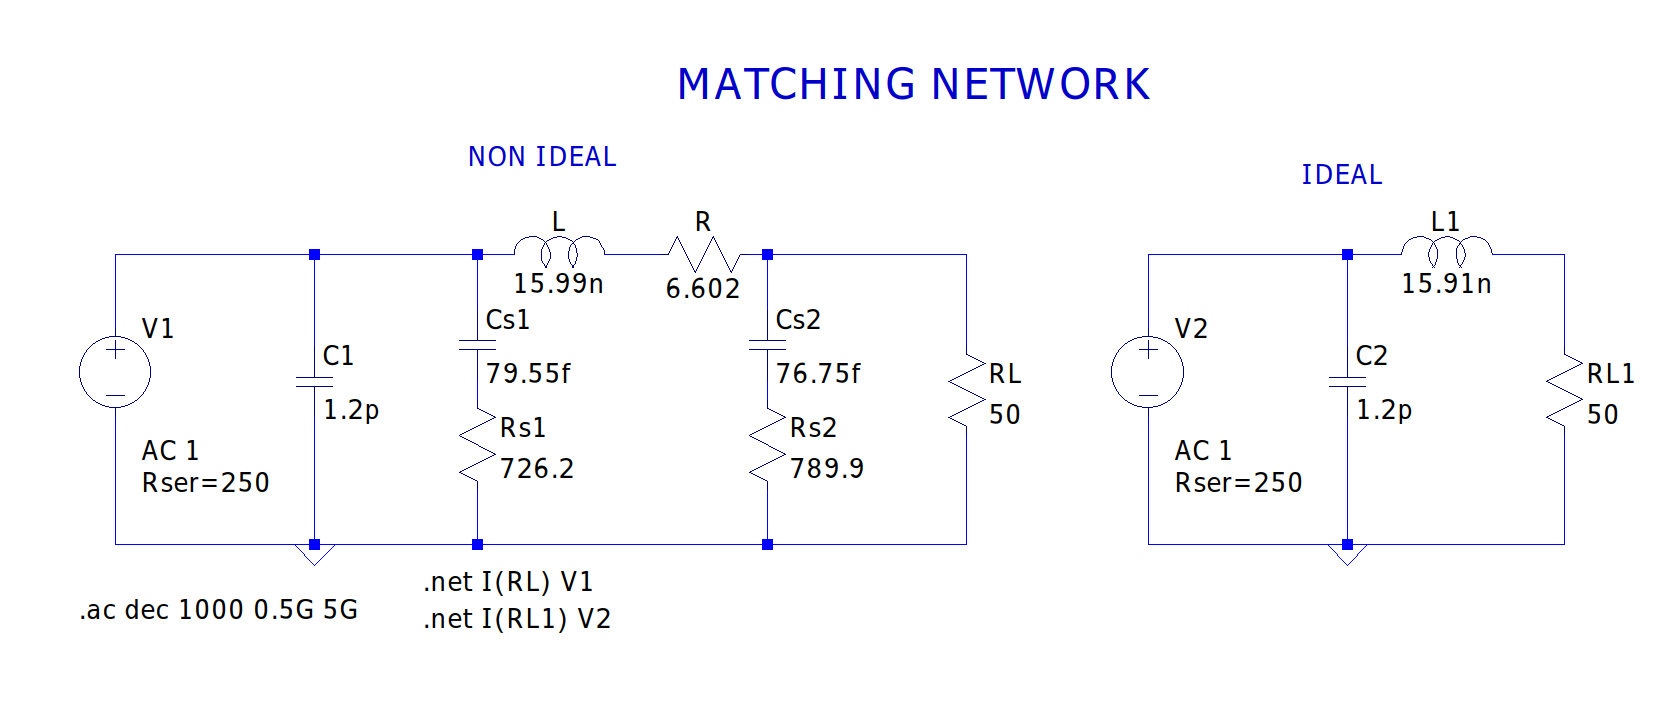
\includegraphics[scale=0.3]{./figs/schematic.png}
\end{figure}
\section*{\hfil S-parameters}
\subsection*{S11, S22 Return Loss}
Port 1 side is \textbf{-23.15dB} and Port 2 side is \textbf{-23.12dB} which also satisfies given constraints.
\begin{figure}[H]
	\centering
	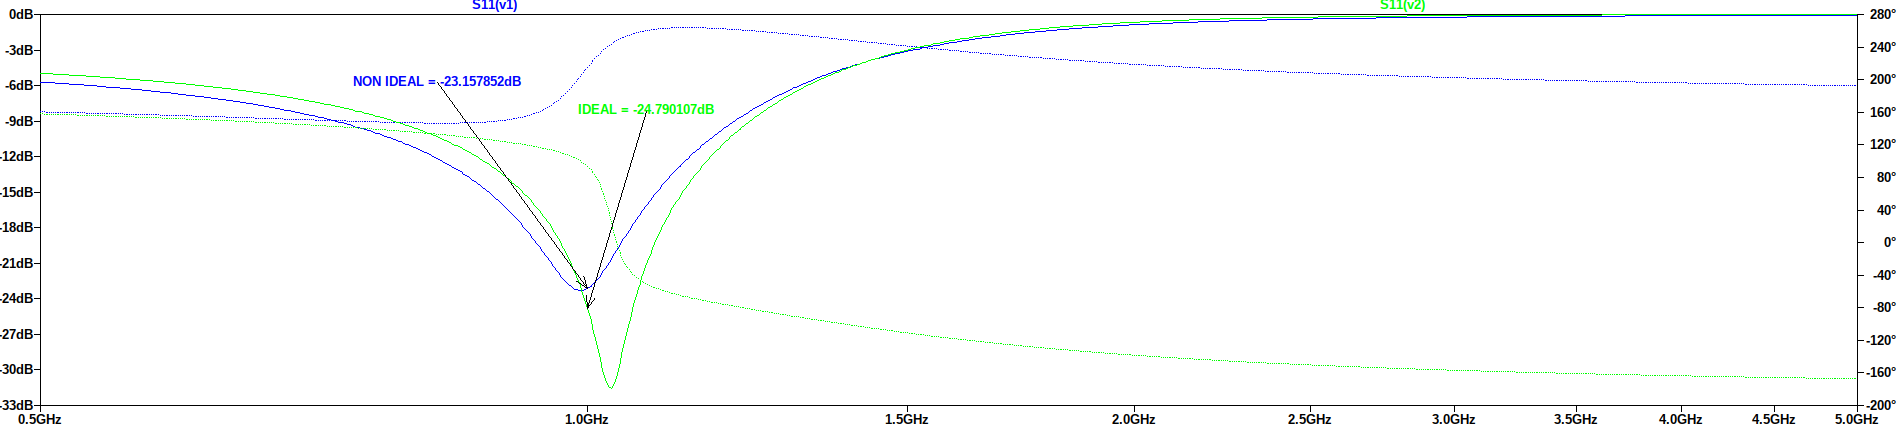
\includegraphics[scale=0.27]{./figs/s11.png}\\
	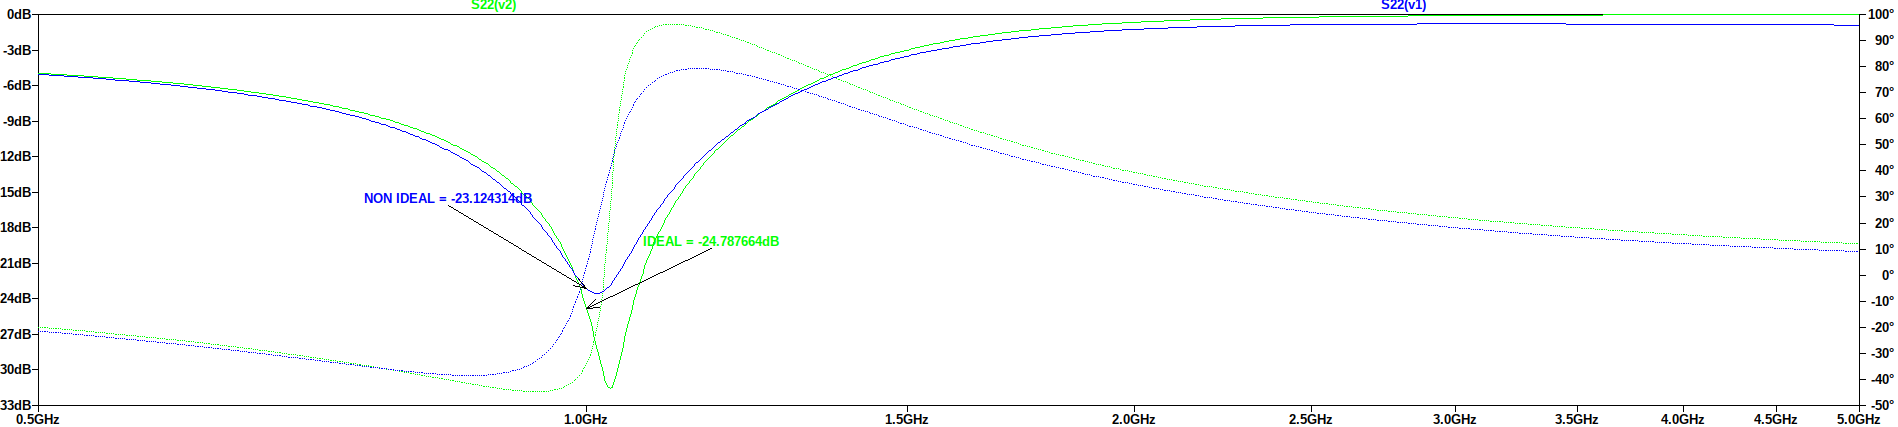
\includegraphics[scale=0.27]{./figs/s22.png}
\end{figure}
\subsection*{Insertion Loss}
Insertion loss here is $\mathbf{-20log|S_{21}|}$ and the same is plotted. After many iterations of inductor design, insertion loss of \textbf{757.4mdB} is obtained.
\begin{figure}[H]
	\centering
	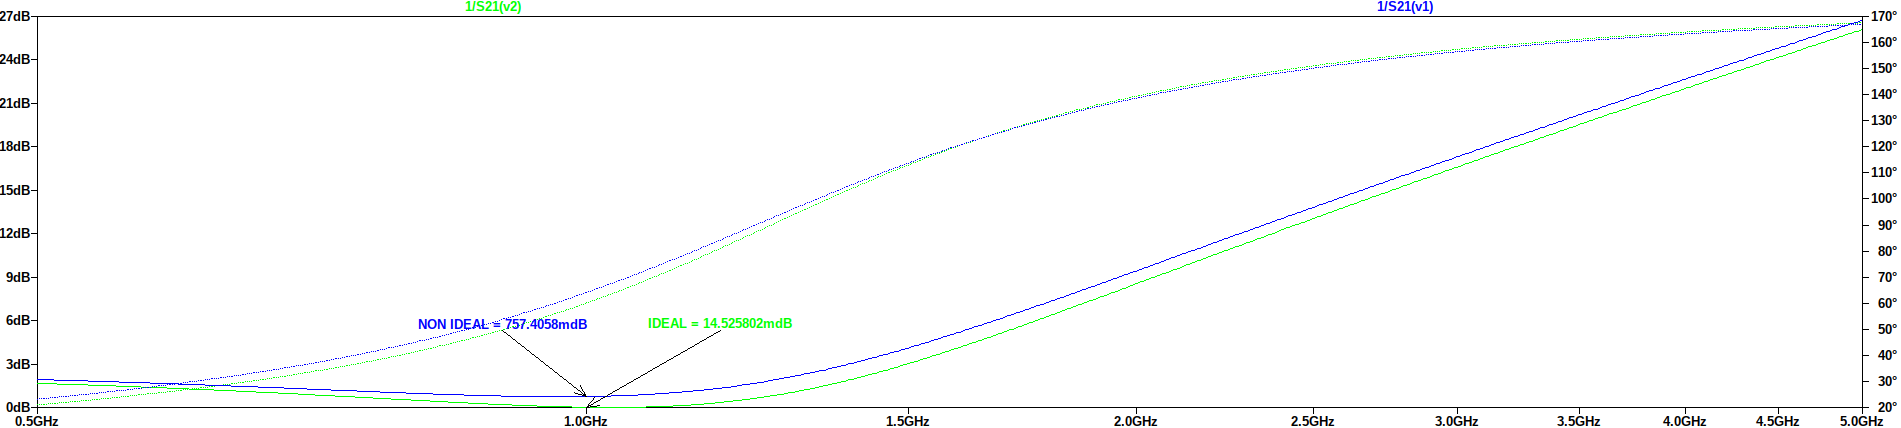
\includegraphics[scale=0.27]{./figs/s21.png}
\end{figure}
\subsection*{S12}\begin{figure}[H]
	\centering
	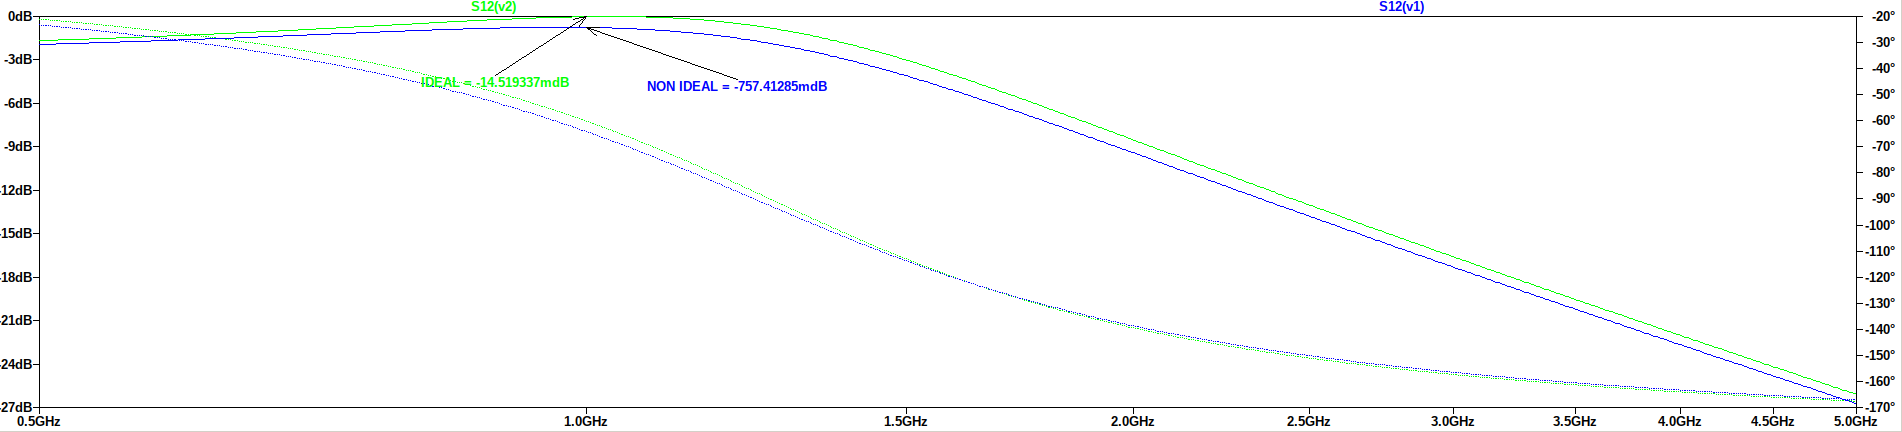
\includegraphics[scale=0.27]{./figs/s12.png}
\end{figure}

\section*{\hfil IDEAL vs NON IDEAL}
\begin{table}[H]
\centering
\begin{tabular}{||l|l|l|l||}
\hline
\textbf{S-parameters} & \textbf{IDEAL}     & \textbf{NON IDEAL} & \textbf{Metric}            \\
\hline
S11          & \textbf{-24.79dB}  & -23.157dB & \textit{Lower is better.}  \\
\hline
S12          & -14.52mdB & \textbf{-757.4mdB} & \textit{Lower is better.}  \\
\hline
S21          & \textbf{-14.52mdB} & -757.4mdB & \textit{Higher is better.} \\
\hline
S22          & \textbf{-24.79dB}  & -23.12dB  & \textit{Lower is better.} \\
\hline
\end{tabular}
\end{table}
\end{document}